% Provenance (never printed): old premiere S material on magmatic rocks (volcanic
% and plutonic textures and cooling rate; basalt/gabbro, andesite/diorite,
% rhyolite/granite; order of crystallisation, told). Cooling of sheets from
% figdata/grade-11/dyke_cooling.py (Delaney 1986 parameters; kappa from England
% et al. 2007). Fractional crystallisation is Year 2's; metamorphism (contact
% aureoles) is g12.03's: not developed here.
\chapter{Las rocas ígneas}\label{ch:g11:igneous-rocks}

En la costa norte de Irlanda, columnas de piedra apretadas unas contra otras
bajan en escalones hasta el mar: la Calzada del Gigante, un basalto que
se enfrió a partir de una lava. En Yosemite, en California, la pared de
granito de El Capitan se alza unos \qty{900}{m} sobre el fondo del valle, un
único cuerpo de roca de grano grueso. Los dos cristalizaron a partir de un
magma. El basalto se enfrió en la superficie, con cristales demasiado
pequeños para verse; el granito se enfrió a gran profundidad, con cristales
lo bastante grandes para verse, y hoy solo es visible porque las rocas que
tenía encima se han desgastado. Este capítulo lee en los granos de una roca
a qué velocidad, y a qué profundidad, se enfrió.
% ledger: photo:g11-giants-causeway, photo:g11-el-capitan, tulane:intrusions

\begin{omfigure}
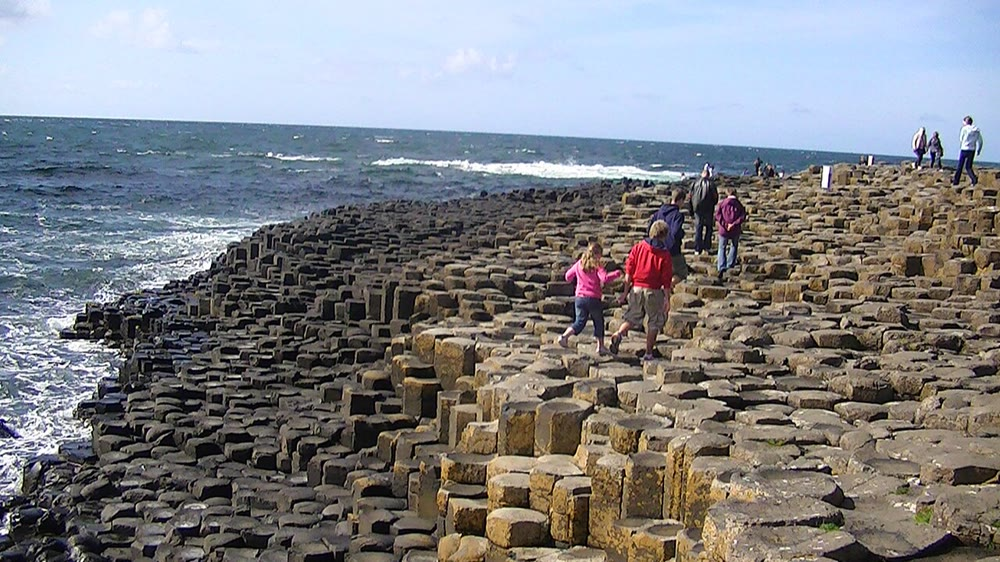
\includegraphics[height=4.3cm]{images/book2/g11-bishop-giants-causeway.jpg}\hspace{0.04\linewidth}%
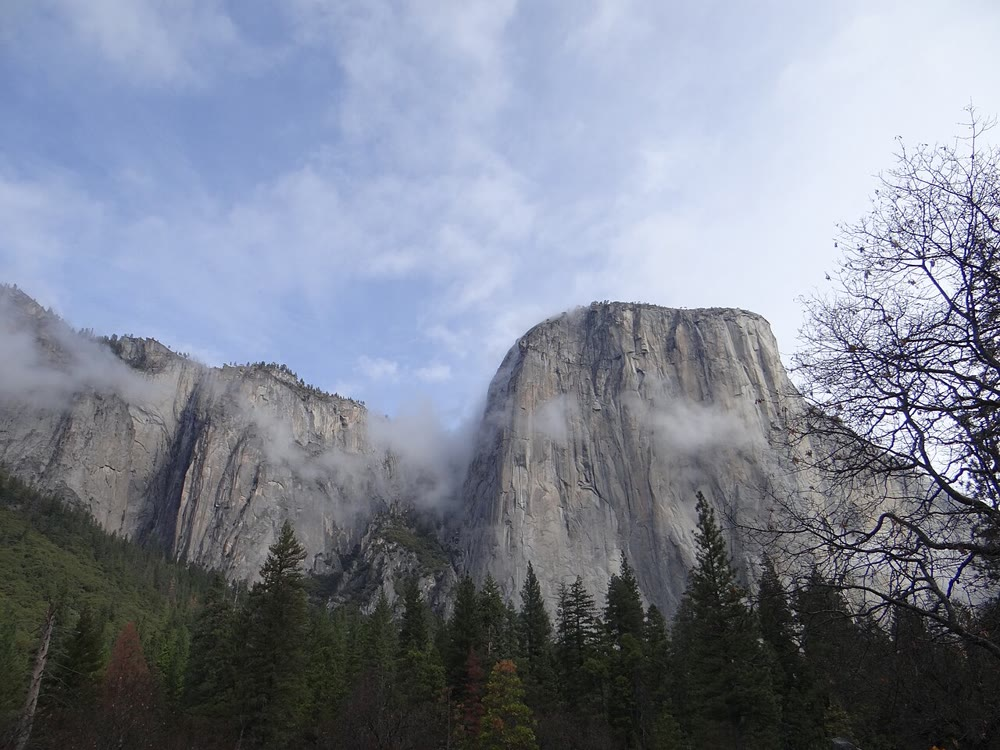
\includegraphics[height=4.3cm]{images/book2/g11-usgs-el-capitan.jpg}

{\small A la izquierda: columnas de basalto de la Calzada del Gigante, en
Irlanda del Norte. Fotografía de Adam Bishop (CC~BY-SA~3.0). A la derecha:
El Capitan, en Yosemite, California, una pared de granito de unos
\qty{900}{m} de altura. Fotografía del U.S. Geological Survey (CC0).}
\end{omfigure}
% ledger: photo:g11-giants-causeway, photo:g11-el-capitan

\begin{recall}
El magma es roca fundida bajo la superficie; sale en erupción como lava, de
forma tranquila o explosiva (Libro 1, año 7). Una roca ígnea es la que se
forma cuando una roca fundida se enfría y se solidifica (Libro 1, año 6). El basalto es una \omterm{def:g11:igneous-rocks:volcanic-plutonic}{roca volcánica} oscura, y el granito, una
roca clara formada por feldespato, cuarzo y mica (Libro 1, año 6). La
\omterm{def:g11:ocean-ridges:peridotite}{peridotita} del manto se funde en parte al ascender bajo una dorsal, y da el
basalto y el \omterm{def:g11:ocean-ridges:gabbro}{gabro} de la \omterm{def:g11:ocean-ridges:oceanic-lithosphere}{corteza oceánica} (el \cref{ch:g11:ocean-ridges}). Los
\omterm{def:g11:minerals:rock-forming}{silicatos formadores de rocas} son el olivino, los piroxenos, los anfíboles,
las micas, los feldespatos y el cuarzo; los feldespatos son el feldespato
potásico y la plagioclasa, una serie que va de rica en calcio a rica en sodio
(el \cref{ch:g11:minerals}). El calor se propaga por conducción a una
distancia de unos $\sqrt{\kappa t}$ en un tiempo $t$, donde $\kappa$ es la
difusividad térmica (el \cref{ch:g11:subduction-zones}).
\end{recall}
% ledger: tulane:ridge-rocks, england:kelvin

\section{Rocas volcánicas y rocas plutónicas}

\begin{definition}[Roca volcánica; roca plutónica]\label{def:g11:igneous-rocks:volcanic-plutonic}
Una roca ígnea, formada por la cristalización de un magma, es
\emph{volcánica}\index{roca volcanica@roca volcánica}
(o extrusiva) cuando el magma se solidificó en la superficie de la Tierra,
como lava, y \emph{plutónica}\index{roca plutonica@roca plutónica} (o intrusiva) cuando
cristalizó en profundidad, dentro de otras rocas.
\end{definition}
% ledger: tulane:magma-types

La diferencia se nota en el tamaño de los cristales. Un cristal crece
añadiendo átomos tomados del líquido que lo rodea, y eso lleva tiempo. En la
superficie, una lava pierde deprisa su calor en el aire o en el agua: el
material lanzado al aire o al agua se enfría en segundos, y una colada de lava,
en días o semanas. En profundidad, las rocas de alrededor están calientes y el
magma pierde su calor despacio: una \omterm{def:g11:igneous-rocks:intrusion}{intrusión} poco profunda se enfría en
meses o años, y una grande y profunda puede tardar millones de años. Un
enfriamiento rápido da muchos cristales pequeños, o ninguno; un enfriamiento
lento da menos cristales, y mucho más grandes.
% ledger: tulane:cooling-times, tulane:textures

\begin{definition}[Textura]\label{def:g11:igneous-rocks:texture}
La \emph{textura}\index{textura (de una roca)} de una roca es el tamaño, la
forma y la disposición de sus granos. Una roca ígnea es \emph{vítrea} cuando
no tiene cristales, \emph{de grano fino} cuando sus cristales son demasiado
pequeños para distinguirse a simple vista, y \emph{de grano grueso} cuando
pueden verse todos.
\end{definition}
% ledger: tulane:textures

Una lava enfriada de golpe antes de que pueda crecer ningún cristal se
convierte en un vidrio: la obsidiana, negra y vítrea, se rompe con la
\omterm{def:g11:minerals:cleavage}{fractura} concoidea de una botella. El basalto es de grano fino: en la mano no
pueden identificarse sus minerales, e incluso en \omterm{def:g11:minerals:thin-section}{lámina delgada} los cristales
son pequeños (el basalto del \cref{ch:g11:minerals}). El granito, el \omterm{def:g11:ocean-ridges:gabbro}{gabro} y
la \omterm{def:g11:igneous-rocks:rock-names}{diorita} son de grano grueso: se ve cada grano.
% ledger: photo:g11-obsidian, photo:g11-basalt, tulane:textures

\begin{definition}[Fenocristal; porfídica]\label{def:g11:igneous-rocks:porphyritic}
Un \emph{fenocristal}\index{fenocristal} es un cristal grande inmerso en una
masa de cristales mucho más pequeños o de vidrio, la \emph{matriz}. Una roca
con fenocristales es \emph{porfídica}\index{porfidica@porfídica}.
\end{definition}
% ledger: tulane:textures

Una \omterm{def:g11:igneous-rocks:texture}{textura} \omterm{def:g11:igneous-rocks:porphyritic}{porfídica} registra dos etapas de enfriamiento: primero lenta, en
profundidad, mientras los \omterm{def:g11:igneous-rocks:porphyritic}{fenocristales} crecían en un magma todavía casi todo
líquido; luego rápida, cuando el magma ascendió y salió en erupción, o se
inyectó en una roca fría, y el resto del líquido se solidificó formando la
matriz.
% ledger: tulane:textures

\begin{omfigure}
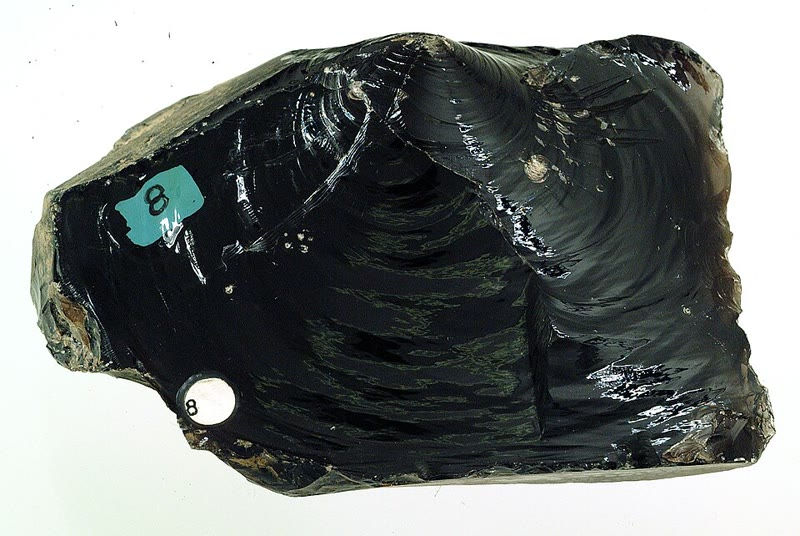
\includegraphics[height=2.75cm]{images/book2/g11-geodil-obsidian.jpg}\hfill
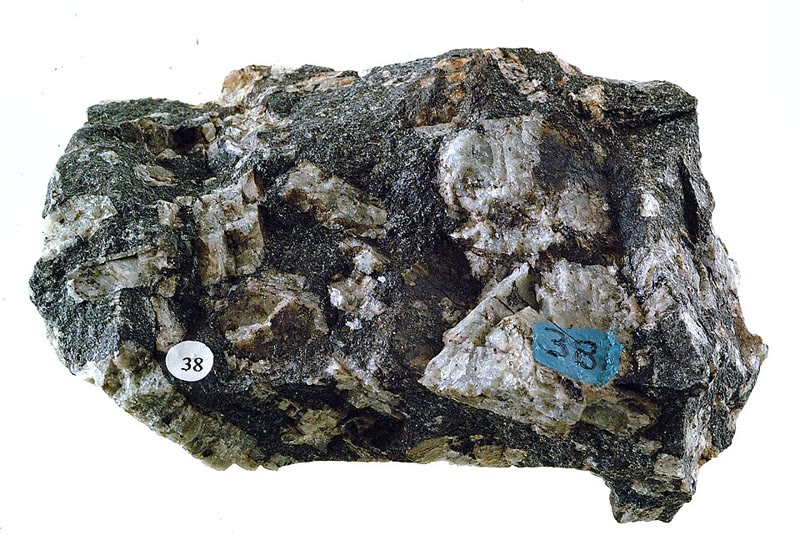
\includegraphics[height=2.75cm]{images/book2/g11-geodil-diabase-porphyry.jpg}\hfill
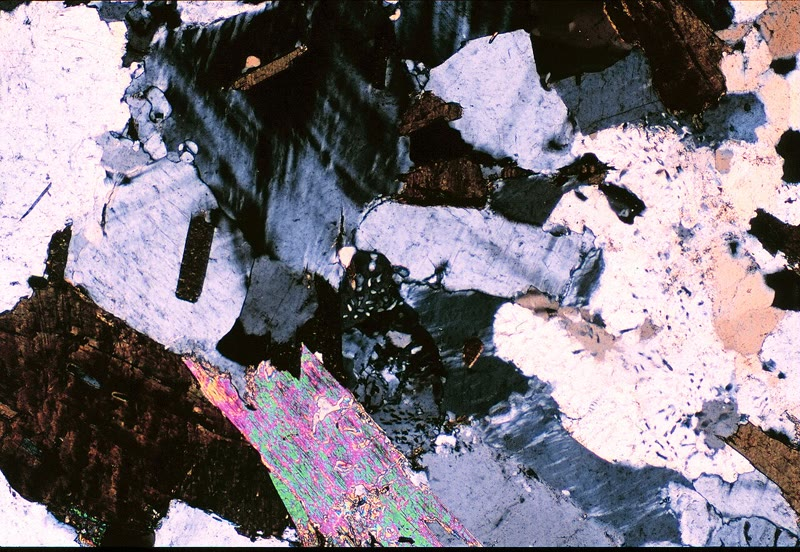
\includegraphics[height=2.75cm]{images/book2/g11-geodil-granite-xpl.jpg}\hfill
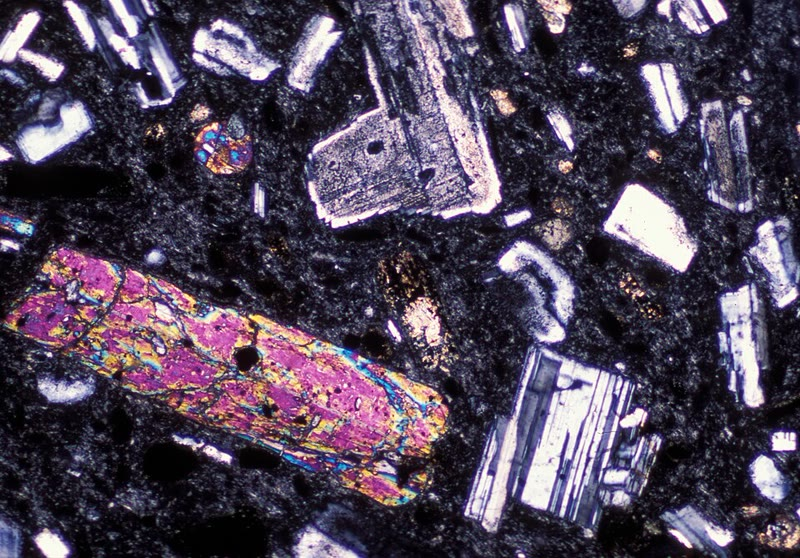
\includegraphics[height=2.75cm]{images/book2/g11-geodil-andesite-xpl.jpg}

{\small De izquierda a derecha: obsidiana, un vidrio volcánico, con su
\omterm{def:g11:minerals:cleavage}{fractura} concoidea curva (\qty{9.5}{cm} de ancho); una roca \omterm{def:g11:igneous-rocks:porphyritic}{porfídica}, con
\omterm{def:g11:igneous-rocks:porphyritic}{fenocristales} macizos de plagioclasa en una matriz más fina (\qty{9}{cm});
luego dos \omterm{def:g11:minerals:thin-section}{láminas delgadas} entre polarizadores cruzados: un granito, con todos
los granos grandes y trabados ---biotita parda, una moscovita de colores
vivos, plagioclasa con bandas, cuarzo gris y blanco---; una \omterm{def:g11:igneous-rocks:rock-names}{andesita}, con
\omterm{def:g11:igneous-rocks:porphyritic}{fenocristales} de plagioclasa y anfíbol en una matriz de grano fino.
Fotografías de Twyla Baker, Mike Davis y Darla Sondrol, Geology Digital Image
Library (CC0).}
\end{omfigure}
% ledger: photo:g11-obsidian, photo:g11-diabase-porphyry, photo:g11-granite-xpl, photo:g11-andesite-xpl

\section{Dar nombre a las rocas ígneas}

La segunda clave de una roca ígnea es su química, y sobre todo su contenido
de sílice, \ce{SiO2}, que en los magmas comunes va de alrededor del
\qty{45}{\percent} a alrededor del \qty{75}{\percent} de la masa.

\begin{definition}[Máfico; intermedio; félsico]\label{def:g11:igneous-rocks:felsic-mafic}
Un magma, o la roca que forma, es \emph{máfico}\index{mafico@máfico} cuando contiene
entre un \qty{45}{\percent} y un \qty{55}{\percent} de \ce{SiO2}, más o menos,
y es rico en hierro, magnesio y calcio; \emph{intermedio}\index{intermedio (roca)}
entre un \qty{55}{\percent} y un \qty{65}{\percent}; \emph{félsico}\index{felsico@félsico}
cuando contiene entre un \qty{65}{\percent} y un \qty{75}{\percent} de \ce{SiO2},
más o menos, y es pobre en hierro, magnesio y calcio pero rico en sodio y
potasio.
\end{definition}
% ledger: tulane:magma-types, earle:magma-oxides

Cada tipo de magma da dos rocas, una \omterm{def:g11:igneous-rocks:volcanic-plutonic}{volcánica} y de grano fino, otra
\omterm{def:g11:igneous-rocks:volcanic-plutonic}{plutónica} y de grano grueso, con la misma química. El basalto y el \omterm{def:g11:ocean-ridges:gabbro}{gabro} son
la pareja \omterm{def:g11:igneous-rocks:felsic-mafic}{máfica}, que ya apareció con la \omterm{def:g11:ocean-ridges:oceanic-lithosphere}{corteza oceánica}; el granito es la
\omterm{def:g11:igneous-rocks:volcanic-plutonic}{roca plutónica} \omterm{def:g11:igneous-rocks:felsic-mafic}{félsica}. Tres nombres completan el conjunto.

\begin{definition}[Andesita; diorita; riolita]\label{def:g11:igneous-rocks:rock-names}
La \emph{andesita}\index{andesita} y la \emph{diorita}\index{diorita} son la
\omterm{def:g11:igneous-rocks:volcanic-plutonic}{roca volcánica} y la \omterm{def:g11:igneous-rocks:volcanic-plutonic}{roca plutónica} de composición \omterm{def:g11:igneous-rocks:felsic-mafic}{intermedia}, formadas sobre
todo por plagioclasa con anfíbol o piroxeno. La \emph{riolita}\index{riolita}
es la \omterm{def:g11:igneous-rocks:volcanic-plutonic}{roca volcánica} de composición \omterm{def:g11:igneous-rocks:felsic-mafic}{félsica}, el equivalente de grano fino del
granito.
\end{definition}
% ledger: tulane:magma-types, earle:bowen, photo:g11-andesite, photo:g11-diorite

\begin{omfigure}
\begin{tikzpicture}[font=\footnotesize, x=0.4cm]
  % columns: SiO2 45 to 75 % mapped to x = 45 to 75 (0.4 cm per %)
  \begin{scope}[xshift=-18cm]
  \fill[omLithBasalt!45] (45,0) rectangle (55,2.4);
  \fill[omLithBasalt!20] (55,0) rectangle (65,2.4);
  \fill[omLithGranite!45] (65,0) rectangle (75,2.4);
  \draw[black!60] (45,0) rectangle (75,2.4);
  \draw[black!60] (55,0) -- (55,2.4); \draw[black!60] (65,0) -- (65,2.4);
  \draw[black!60] (45,1.2) -- (75,1.2);
  \foreach \x/\a/\b in {50/basalto/gabro, 60/andesita/diorita, 70/riolita/granito}{
    \node[font=\small\bfseries, text height=1.6ex, text depth=0.3ex] at (\x,1.8) {\a};
    \node[font=\small\bfseries, text height=1.6ex, text depth=0.3ex] at (\x,0.6) {\b};}
  \node[anchor=east, align=right] at (44.4,1.8) {de grano fino\\(volcánica)};
  \node[anchor=east, align=right] at (44.4,0.6) {de grano grueso\\(plutónica)};
  \node[anchor=south] at (50,2.45) {máfica};
  \node[anchor=south] at (60,2.45) {intermedia};
  \node[anchor=south] at (70,2.45) {félsica};
  % minerals (a drawing: where each mineral is common)
  \foreach \y/\a/\b/\m/\c in {-0.55/45.2/52/olivino/omLithBasalt!80!black,
      -1.15/45.2/61/piroxeno/omLithBasalt!65!black,
      -1.75/52/69/anfíbol/black!60,
      -2.35/57/74.8/biotita/black!75,
      -2.95/45.2/72/plagioclasa/omDef!45,
      -3.55/63/74.8/feldespato potásico/omLithGranite!90!red,
      -4.15/64/74.8/cuarzo/black!20,
      -4.75/68/74.8/moscovita/black!35}{
    \fill[\c] (\a,\y) .. controls ({\a+1.2},{\y+0.22}) and ({\b-1.2},{\y+0.22}) .. (\b,\y)
              .. controls ({\b-1.2},{\y-0.22}) and ({\a+1.2},{\y-0.22}) .. (\a,\y) -- cycle;
    \node[anchor=east] at (44.4,\y) {\m};}
  \node[font=\scriptsize, text=black!75] at (50,-2.95) {rica en calcio};
  \node[font=\scriptsize, text=omDef!80!black, anchor=west] at (72.3,-2.95) {rica en sodio};
  % SiO2 axis
  \draw[-{Stealth[length=4pt]}] (45,-5.35) -- (75.8,-5.35);
  \foreach \x in {45,50,...,75} {\draw (\x,-5.35) -- (\x,-5.45); \node[anchor=north] at (\x,-5.45) {\x};}
  \node[anchor=north] at (60,-5.85) {\ce{SiO2} (\unit{\percent} de la masa)};
  \draw[black!30, dashed] (55,0) -- (55,-5.35); \draw[black!30, dashed] (65,0) -- (65,-5.35);
  \end{scope}
\end{tikzpicture}

{\small Nombres de las rocas ígneas comunes (un dibujo). Columnas: el
contenido de sílice del magma; filas: rocas de grano fino (\omterm{def:g11:igneous-rocks:volcanic-plutonic}{volcánicas}) y de
grano grueso (\omterm{def:g11:igneous-rocks:volcanic-plutonic}{plutónicas}). Debajo, dónde es frecuente cada mineral formador de
rocas: olivino y piroxeno en las rocas \omterm{def:g11:igneous-rocks:felsic-mafic}{máficas}, con plagioclasa rica en
calcio; anfíbol y plagioclasa en las rocas \omterm{def:g11:igneous-rocks:felsic-mafic}{intermedias}; feldespato potásico,
cuarzo, plagioclasa rica en sodio y micas en las rocas \omterm{def:g11:igneous-rocks:felsic-mafic}{félsicas}. Los límites
son graduales.}
\end{omfigure}
% ledger: tulane:magma-types, earle:bowen, earle:magma-oxides, photo:g11-andesite, photo:g11-diorite, photo:g11-granite, nps:granite-minerals

\begin{method}[Dar nombre a una roca ígnea]\label{met:g11:igneous-rocks:naming}
\begin{enumerate}
  \item Observa la \omterm{def:g11:igneous-rocks:texture}{textura}: vítrea, de grano fino o de grano grueso;
        \omterm{def:g11:igneous-rocks:porphyritic}{porfídica} o no. De grano fino o vítrea significa \omterm{def:g11:igneous-rocks:volcanic-plutonic}{volcánica} (o una
        \omterm{def:g11:igneous-rocks:intrusion}{intrusión} pequeña, enfriada deprisa); de grano grueso significa \omterm{def:g11:igneous-rocks:volcanic-plutonic}{plutónica}.
  \item Identifica los minerales que pueden verse
        (el \cref{met:g11:minerals:identify}): el cuarzo y el feldespato
        potásico apuntan a \omterm{def:g11:igneous-rocks:felsic-mafic}{félsica}, el anfíbol con plagioclasa a \omterm{def:g11:igneous-rocks:felsic-mafic}{intermedia}, el
        olivino y el piroxeno a \omterm{def:g11:igneous-rocks:felsic-mafic}{máfica}. En una roca de grano fino, usa los
        \omterm{def:g11:igneous-rocks:porphyritic}{fenocristales}, el color de la matriz ---oscura en las \omterm{def:g11:igneous-rocks:felsic-mafic}{máficas}, clara en
        las félsicas--- como indicio, o un análisis químico.
  \item Lee el nombre en el cruce de la fila y la columna del
        cuadro.
\end{enumerate}
\end{method}

\begin{example}[Dos basaltos]
Una roca oscura de una colada de lava es de grano fino en toda su masa; otra,
del mismo volcán, muestra granos verdes de olivino de unos milímetros en una
matriz oscura. Las dos son \omterm{def:g11:igneous-rocks:felsic-mafic}{máficas} y de grano fino: las dos son basaltos. La
segunda es un basalto porfídico: su olivino creció primero, despacio, en el
magma bajo el volcán, antes de que la lava saliera en erupción y se
solidificara a su alrededor.
\end{example}
% ledger: photo:g11-olivine, earle:bowen, tulane:textures

\begin{omfigure}
\makebox[0.32\linewidth]{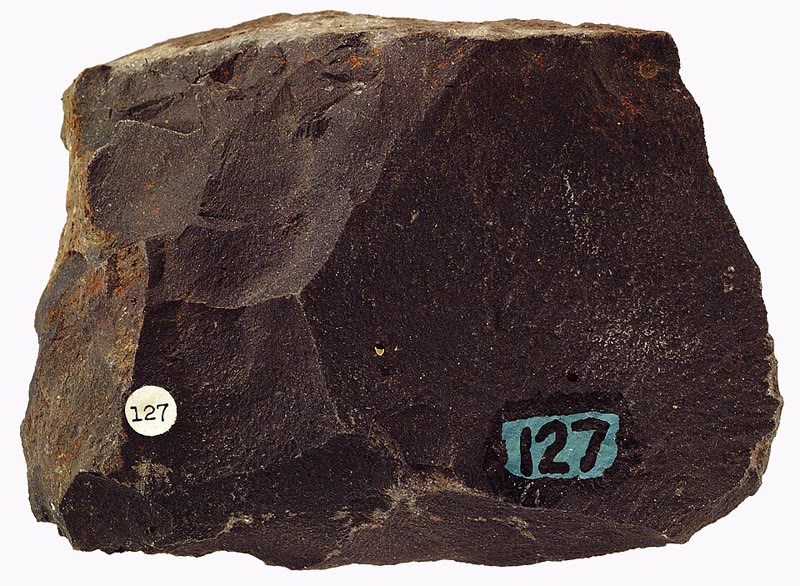
\includegraphics[height=2.9cm]{images/book2/g11-geodil-basalt.jpg}}\hfill
\makebox[0.32\linewidth]{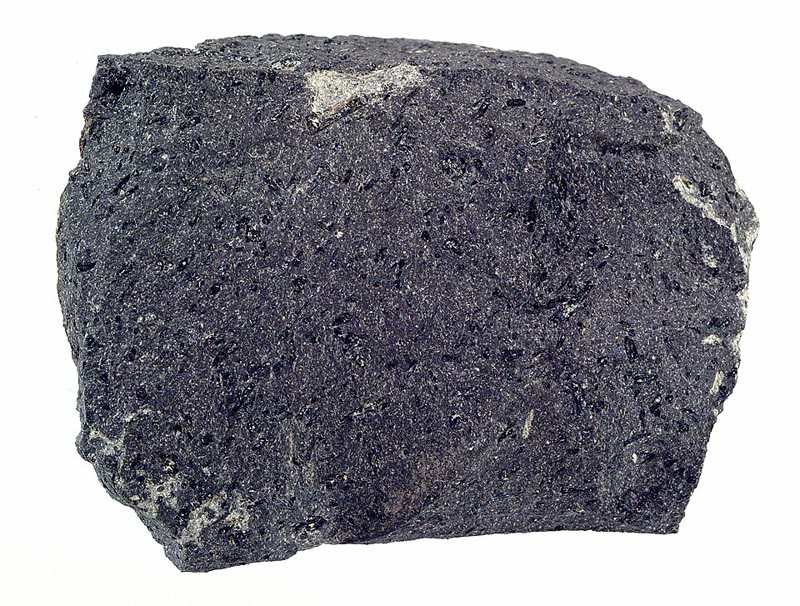
\includegraphics[height=2.9cm]{images/book2/g11-geodil-andesite.jpg}}\hfill
\makebox[0.32\linewidth]{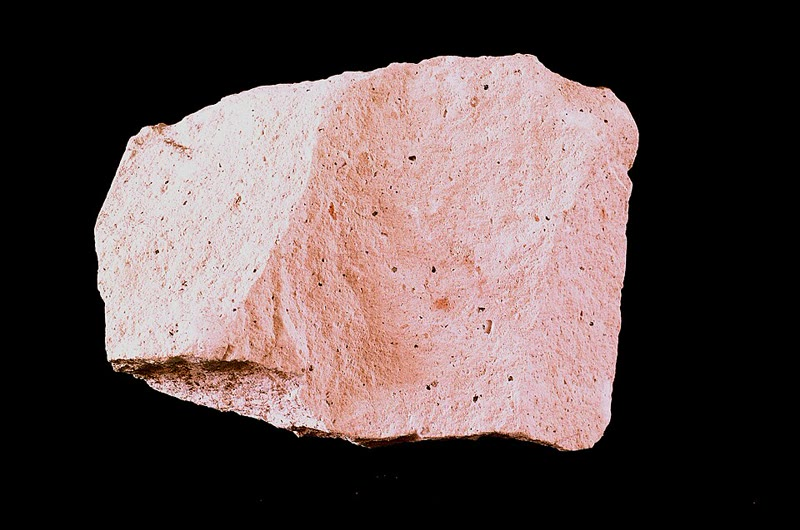
\includegraphics[height=2.9cm]{images/book2/g11-geodil-rhyolite.jpg}}

\smallskip
\makebox[0.32\linewidth]{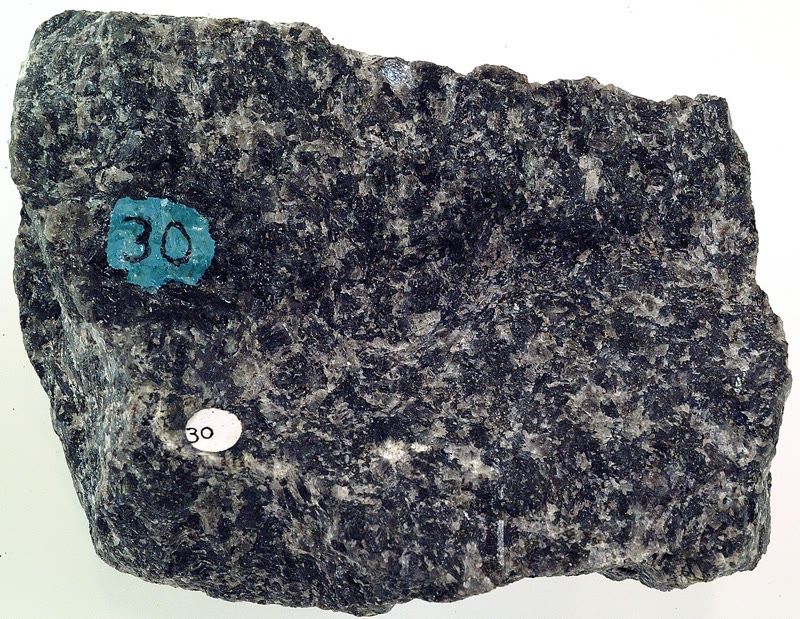
\includegraphics[height=2.9cm]{images/book2/g11-geodil-gabbro.jpg}}\hfill
\makebox[0.32\linewidth]{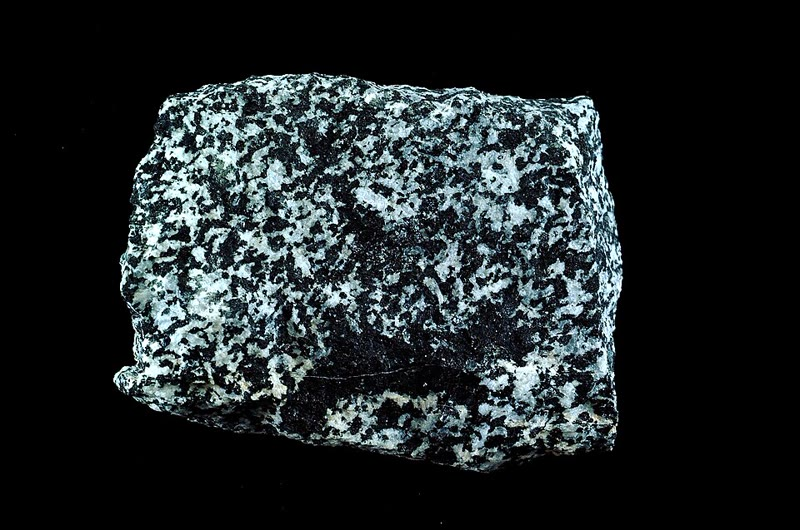
\includegraphics[height=2.9cm]{images/book2/g11-geodil-diorite.jpg}}\hfill
\makebox[0.32\linewidth]{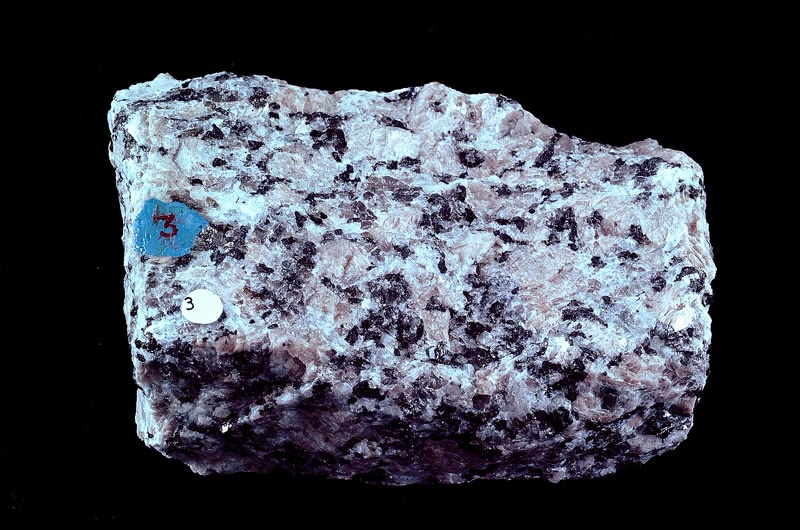
\includegraphics[height=2.9cm]{images/book2/g11-geodil-granite.jpg}}

{\small Las tres parejas de rocas ígneas, de \omterm{def:g11:igneous-rocks:felsic-mafic}{máfica} a \omterm{def:g11:igneous-rocks:felsic-mafic}{félsica} de izquierda a
derecha: \omterm{def:g11:igneous-rocks:volcanic-plutonic}{volcánicas} arriba, \omterm{def:g11:igneous-rocks:volcanic-plutonic}{plutónicas} abajo. Arriba: un basalto de grano
fino; una \omterm{def:g11:igneous-rocks:rock-names}{andesita}, con pequeños cristales de anfíbol en una matriz de grano
fino (unos \qty{10}{cm}); una \omterm{def:g11:igneous-rocks:rock-names}{riolita} rosa. Abajo: \omterm{def:g11:ocean-ridges:gabbro}{gabro} (\qty{9}{cm});
\omterm{def:g11:igneous-rocks:rock-names}{diorita}, con hornblenda negra y plagioclasa vítrea (\qty{10}{cm}); un granito
grueso con grandes feldespatos potásicos de color rosa pálido, plagioclasa
gris, cuarzo, biotita y hornblenda (\qty{10}{cm}). Fotografías de Nessa Eull,
Twyla Baker, Joseph H.~Hartman, Darla Sondrol y Dexter Perkins, Geology
Digital Image Library (CC0).}
\end{omfigure}
% ledger: photo:g11-basalt, photo:g11-andesite, photo:g11-rhyolite, photo:g11-gabbro, photo:g11-diorite, photo:g11-granite

\section{El orden de cristalización}

Un magma no se solidifica a una sola temperatura, como el agua. Sus minerales
aparecen uno tras otro a medida que se enfría, cada uno en su propio intervalo
de temperatura, de modo que un magma que se enfría puede contener cristales y
seguir siendo casi todo líquido.

\begin{history}[Los experimentos de Bowen]
Norman L.~Bowen (1887--1956) entró en el Geophysical Laboratory de la
Carnegie Institution de Washington en 1912. Trabajando sobre todo con magmas
basálticos, fundía una roca en un horno, la dejaba enfriarse despacio hasta
una temperatura elegida para que se formaran algunos minerales, y luego la
templaba, enfriándola tan deprisa que el líquido restante se convertía en un
vidrio. Al microscopio, los cristales mostraban qué minerales se habían
formado por encima de esa temperatura. Repetido a temperaturas cada vez más
bajas, el experimento dio el orden en que aparecen los minerales. Bowen
publicó este orden como una serie de reacción en 1922, y su libro
\emph{The Evolution of the Igneous Rocks} en 1928.
\end{history}
% ledger: carnegie:bowen, earle:bowen

\begin{omfigure}
\begin{tikzpicture}[font=\footnotesize, box/.style={draw=black!60, rounded corners=2pt, fill=#1, minimum width=3.0cm, minimum height=0.62cm, align=center}]
  \node[box=omLithBasalt!45] (ol) at (0,0) {olivino};
  \node[box=omLithBasalt!35] (px) at (0,-1.1) {piroxeno};
  \node[box=black!15] (am) at (0,-2.2) {anfíbol};
  \node[box=black!25] (bi) at (0,-3.3) {biotita};
  \draw[-{Stealth[length=4pt]}, line width=0.8pt] (ol) -- (px);
  \draw[-{Stealth[length=4pt]}, line width=0.8pt] (px) -- (am);
  \draw[-{Stealth[length=4pt]}, line width=0.8pt] (am) -- (bi);
  \node[align=center, anchor=south] at (0,0.45) {\textbf{rama discontinua}\\cada mineral reacciona con el líquido\\y da el siguiente};
  % continuous branch: a wedge from Ca-rich to Na-rich
  \fill[left color=omDef!55, right color=omDef!12, shading angle=180] (5.0,-0.9) -- (6.6,-0.9) -- (6.6,-3.5) -- (5.0,-3.5) -- cycle;
  \shade[top color=omDef!60, bottom color=omDef!10, draw=black!60, rounded corners=2pt] (4.3,-0.85) rectangle (7.3,-3.55);
  \node[align=center] at (5.8,-1.3) {plagioclasa\\rica en calcio};
  \node[align=center] at (5.8,-3.15) {plagioclasa\\rica en sodio};
  \draw[-{Stealth[length=4pt]}, line width=0.8pt] (5.8,-1.65) -- (5.8,-2.7);
  \node[align=center, anchor=south] at (5.8,0.45) {\textbf{rama continua}\\la plagioclasa cambia\\gradualmente};
  % last minerals
  \node[box=omLithGranite!45, minimum width=7.6cm] (last) at (2.9,-4.75) {feldespato potásico, cuarzo, (moscovita)};
  \draw[-{Stealth[length=4pt]}, line width=0.8pt] (bi) -- (bi |- last.north);
  \draw[-{Stealth[length=4pt]}, line width=0.8pt] (5.8,-3.55) -- (5.8,-4.43);
  % temperature arrow
  \draw[-{Stealth[length=5pt]}, line width=1pt, omThm] (-2.6,0.3) -- (-2.6,-4.9);
  \node[anchor=east, align=right, text=omThm] at (-2.75,0.1) {primero,\\\qtyrange{1200}{1300}{\degreeCelsius}};
  \node[anchor=east, align=right, text=omThm] at (-2.75,-4.7) {al final, unos\\\qtyrange{750}{800}{\degreeCelsius}};
  \node[anchor=east, align=right, text=omThm] at (-2.75,-2.3) {temperatura\\descendente};
\end{tikzpicture}

{\small El orden en que cristalizan los minerales a partir de un magma que se
enfría (la serie de reacción de Bowen, un dibujo). El olivino se forma
primero; la plagioclasa empieza más o menos donde empieza el piroxeno, rica en
calcio al principio y luego cada vez más rica en sodio. El feldespato
potásico, el cuarzo y a veces la moscovita se forman al final, a partir de lo
que queda de un líquido rico en sílice.}
\end{omfigure}
% ledger: earle:bowen

La palabra \emph{reacción} importa. El olivino solo es estable a alta
temperatura: a medida que el magma se enfría, los cristales de olivino
reaccionan con la sílice del líquido y se convierten en piroxeno,
\[
  \ce{Mg2SiO4 + SiO2 -> 2 MgSiO3},
\]
y así sucesivamente a lo largo de la rama, mientras quede sílice en el
líquido. En la otra rama, los cristales de plagioclasa siguen creciendo, pero
cada nueva capa es más rica en sodio que la anterior: un cristal de
plagioclasa puede estar zonado, desde un núcleo rico en calcio hasta un borde
rico en sodio, como los \omterm{def:g11:igneous-rocks:porphyritic}{fenocristales} de plagioclasa de la \omterm{def:g11:igneous-rocks:rock-names}{andesita} de arriba.
% ledger: earle:bowen, photo:g11-andesite-xpl

La serie explica el cuadro. Un magma \omterm{def:g11:igneous-rocks:felsic-mafic}{máfico} se queda pronto sin sílice:
cristaliza olivino, piroxeno y plagioclasa rica en calcio, y da un \omterm{def:g11:ocean-ridges:gabbro}{gabro} si
se enfría despacio en profundidad, o un basalto si se enfría deprisa en la
superficie. Solo un magma rico en sílice llega hasta el final de la serie y
forma feldespato potásico y cuarzo: los minerales del granito y de la \omterm{def:g11:igneous-rocks:rock-names}{riolita}.
Cómo cambia un magma su composición por el camino, cuando sus primeros
cristales se separan del líquido, es materia del segundo año de universidad.
% ledger: earle:bowen, tulane:bowen

\section{Las intrusiones}

El magma asciende porque es menos denso que las rocas que lo rodean, y se abre
paso por las fracturas ensanchándolas. Gran parte de él nunca llega a la
superficie: cristaliza en la corteza en forma de intrusiones, que solo se ven
cuando la erosión ha eliminado las rocas de encima.
% ledger: tulane:intrusions

\begin{definition}[Dique; filón capa; plutón]\label{def:g11:igneous-rocks:intrusion}
Una \emph{intrusión}\index{intrusion@intrusión} es un cuerpo de roca ígnea que cristalizó
dentro de otras rocas. Un \emph{dique}\index{dique} es una lámina de roca
ígnea que corta las capas o las estructuras de las rocas en las que se
intruye; un \emph{filón capa}\index{filon capa@filón capa} es una lámina paralela a las
capas, situada entre ellas. Un \emph{plutón}\index{pluton@plutón} es una intrusión
grande, de cualquier forma, formada en profundidad; muchos plutones unidos
forman un batolito (el \cref{ch:g12:subduction-magmatism}).
\end{definition}
% ledger: tulane:intrusions

Los \omterm{def:g11:igneous-rocks:intrusion}{diques} suelen tener menos de \qty{20}{m} de anchura, y los \omterm{def:g11:igneous-rocks:intrusion}{filones capa},
menos de \qty{50}{m} de espesor; un \omterm{def:g11:igneous-rocks:intrusion}{filón capa} suele estar alimentado por un
\omterm{def:g11:igneous-rocks:intrusion}{dique}. Los \omterm{def:g11:igneous-rocks:intrusion}{diques} y los \omterm{def:g11:igneous-rocks:intrusion}{filones capa} poco profundos se enfrían deprisa: son de
grano fino, a veces porfídicos. En contacto con la roca fría en la que se
intruyen, sus bordes se enfrían todavía más deprisa y son de grano aún más
fino que su centro: un \emph{borde enfriado}, la marca de un cuerpo que estaba
caliente cuando se emplazó. Sierra Nevada, en California, donde está
Yosemite, es un batolito: las rocas graníticas cuya densidad se midió en el
\cref{ch:g11:minerals} proceden de unos doscientos de sus \omterm{def:g11:igneous-rocks:intrusion}{plutones}.
% ledger: tulane:intrusions, usgs91:sierra, photo:g11-el-capitan

\begin{omfigure}
\begin{tikzpicture}[font=\footnotesize, scale=0.9]
  % layered host rocks
  \fill[omLithSand] (0,0) rectangle (14,-1.0);
  \fill[omLithShale] (0,-1.0) rectangle (14,-2.0);
  \fill[omLithLime] (0,-2.0) rectangle (14,-3.0);
  \fill[omLithSand] (0,-3.0) rectangle (14,-4.0);
  \fill[omLithShale] (0,-4.0) rectangle (14,-6.4);
  \foreach \y in {-1,-2,-3,-4} \draw[black!35] (0,\y) -- (14,\y);
  % pluton
  \fill[omLithGranite, draw=black!60] (2.2,-6.4) .. controls (2.4,-4.6) and (3.6,-4.1) .. (5.5,-4.15)
     .. controls (7.4,-4.2) and (9.0,-4.5) .. (9.6,-6.4) -- cycle;
  % sill between the limestone and the shale, fed by the dyke
  \fill[omLithBasalt, draw=black!60] (7.3,-1.88) -- (12.6,-1.88) .. controls (12.9,-1.9) and (12.9,-2.1) .. (12.6,-2.12) -- (7.3,-2.12) -- cycle;
  % dyke from the pluton to the volcano
  \fill[omLithBasalt, draw=black!60] (7.0,-4.18) -- (7.3,-4.2) -- (7.3,0) -- (7.0,0) -- cycle;
  % a second dyke cutting across the layers, not reaching the surface
  \fill[omLithBasalt, draw=black!60] (3.9,-4.15) -- (4.15,-4.15) -- (2.95,-0.6) -- (2.75,-0.6) -- cycle;
  % volcano and lava flow
  \fill[black!65] (5.75,0) -- (7.15,1.35) -- (8.55,0) -- cycle;
  \fill[omLithBasalt!80!black] (8.4,0) -- (11.6,0) -- (11.6,0.1) .. controls (10.5,0.16) and (9.2,0.22) .. (8.3,0.15) -- cycle;
  \draw[black!70] (0,0) -- (5.75,0); \draw[black!70] (8.55,0) -- (14,0);
  % labels
  \node[anchor=south] at (7.15,1.4) {volcán};
  \draw[black!60] (10.5,0.15) -- (11.2,0.8); \node[anchor=south west, inner sep=1pt] at (11.2,0.8) {colada de lava};
  \draw[black!60] (7.3,-0.5) -- (8.3,-0.5); \node[anchor=west, fill=omLithSand, inner sep=1pt] at (8.3,-0.5) {dique (corta las capas)};
  \draw[black!60] (11.0,-2.0) -- (11.0,-2.55); \node[anchor=north, fill=omLithLime, inner sep=1pt] at (11.0,-2.55) {filón capa (entre las capas)};
  \draw[black!60] (3.4,-2.5) -- (1.9,-2.5); \node[anchor=east, fill=omLithLime, inner sep=1pt] at (1.9,-2.5) {dique};
  \node[align=center] at (5.9,-5.5) {plutón};
  \node[anchor=east, fill=omLithShale, inner sep=1pt] at (13.85,-5.3) {rocas sedimentarias en capas};
\end{tikzpicture}

{\small Intrusiones (un dibujo, no a escala). Un \omterm{def:g11:igneous-rocks:intrusion}{plutón} cristaliza en
profundidad; los \omterm{def:g11:igneous-rocks:intrusion}{diques} cortan las capas de las rocas que tiene encima, y uno
de ellos alimenta un volcán; un \omterm{def:g11:igneous-rocks:intrusion}{filón capa} se extiende entre dos capas. Solo
la erosión de las rocas de encima deja estos cuerpos al descubierto en la
superficie.}
\end{omfigure}
% ledger: tulane:intrusions

¿Cuánto tarda en cristalizar una \omterm{def:g11:igneous-rocks:intrusion}{intrusión}? Considera una lámina de
magma ---un \omterm{def:g11:igneous-rocks:intrusion}{dique} o un filón capa--- de espesor $b$, que pierde su calor por
conducción hacia la roca de ambos lados. Las únicas magnitudes que marcan el
ritmo son el espesor $b$, en metros, y la difusividad térmica $\kappa$, en
\unit{m^2/s}; el único tiempo que puede construirse con ellas es $b^2/\kappa$.
% ledger: england:kelvin, delaney86:example

\begin{proposition}[El tiempo de enfriamiento de una lámina de magma]\label{prop:g11:igneous-rocks:cooling}
Una lámina de magma de espesor $b$ que se enfría por conducción se solidifica
en un tiempo
\[
  t = C\,\frac{b^2}{\kappa},
\]
donde $\kappa$ es la difusividad térmica de las rocas y $C$ un número fijado
por las temperaturas del magma y de la roca que lo rodea y por el calor que
libera el magma al cristalizar. Duplicar el espesor multiplica el tiempo por
cuatro. (Se admite; el valor de $C$ procede de un modelo calculado.)
\end{proposition}
% ledger: delaney86:properties, delaney86:example

Para un magma basáltico intruido a \qty{1150}{\degreeCelsius} en una roca a
\qty{50}{\degreeCelsius}, que cristaliza por completo a
\qty{950}{\degreeCelsius} y libera \qty{900}{MJ} de calor por cada metro
cúbico que cristaliza, con $\kappa = \qty{1e-6}{m^2/s}$, el modelo da
$C \approx 0.21$. Una lámina de \qty{2}{m} de espesor se solidifica entonces
en unos diez días, un \omterm{def:g11:igneous-rocks:intrusion}{filón capa} de \qty{20}{m} en unos dos años y medio, y
uno de \qty{100}{m} en unos sesenta y cinco años. Sin el calor de
cristalización, los tiempos serían tres veces más cortos: el magma que
cristaliza se mantiene caliente a sí mismo.
% values (dyke_cooling.py): t2_day 9.55, t20_yr 2.61, t100_yr 65.3, latent_factor 2.94; C = 8.2475e7 s / 4e8 s = 0.206
% ledger: delaney86:example, delaney86:properties, england:kelvin

\begin{omfigure}
\begin{tikzpicture}
\begin{axis}[omrecord, name=times, width=0.45\linewidth, height=5.0cm, xmode=log, ymode=log,
  xmin=0.8, xmax=130, ymin=1e-3, ymax=200, xlabel={espesor de la lámina (\unit{m})},
  ylabel={tiempo de solidificación (años)},
  legend style={font=\scriptsize, at={(0.5,-0.4)}, anchor=north, legend columns=2,
    /tikz/every even column/.append style={column sep=4pt}}]
% computed in figdata/grade-11/dyke_cooling.py; ledger: delaney86:*, england:kelvin
\addplot[omThm, line width=1pt, mark=*, mark size=1.4pt] table[x=b, y=t_yr] {figdata/out/grade-11-dyke_cooling-times.dat};
\addplot[omDef, line width=1pt, dashed, mark=o, mark size=1.4pt] table[x=b, y=t0_yr] {figdata/out/grade-11-dyke_cooling-times.dat};
\legend{con calor de cristalización, sin él}
\end{axis}
\begin{axis}[omrecord, at={(times.east)}, anchor=west, xshift=1.6cm, width=0.45\linewidth, height=5.0cm,
  xmin=-28, xmax=28, ymin=0, ymax=1300, xlabel={distancia al centro del filón capa (\unit{m})},
  ylabel={temperatura (\unit{\degreeCelsius})},
  legend style={font=\scriptsize, at={(0.5,-0.4)}, anchor=north, legend columns=4,
    /tikz/every even column/.append style={column sep=4pt}}]
\fill[omLithBasalt!30] (axis cs:-10,0) rectangle (axis cs:10,1300);
\draw[black!50, dashed] (axis cs:-28,950) -- (axis cs:28,950);
\node[font=\scriptsize, anchor=south east, text=black!60] at (axis cs:27,955) {solidus};
\node[font=\scriptsize, anchor=north] at (axis cs:0,1290) {filón capa};
% computed in figdata/grade-11/dyke_cooling.py
\addplot[omProp, line width=0.9pt] table[x=x, y=T1] {figdata/out/grade-11-dyke_cooling-profiles.dat};
\addplot[omThm, line width=0.9pt] table[x=x, y=T2] {figdata/out/grade-11-dyke_cooling-profiles.dat};
\addplot[omDef, line width=0.9pt] table[x=x, y=T3] {figdata/out/grade-11-dyke_cooling-profiles.dat};
\addplot[black, line width=0.9pt] table[x=x, y=T4] {figdata/out/grade-11-dyke_cooling-profiles.dat};
\legend{30 días, 6 meses, 1 año, 2 años}
\end{axis}
\end{tikzpicture}

{\small Una lámina de magma basáltico que se enfría por conducción (modelo
calculado). A la izquierda: el tiempo que tarda en solidificarse, frente a su
espesor, en ejes logarítmicos: una recta de pendiente 2, porque el tiempo
crece como el cuadrado del espesor. A la derecha: temperaturas a través de un
\omterm{def:g11:igneous-rocks:intrusion}{filón capa} de \qty{20}{m} de espesor (sombreado), intruido a
\qty{1150}{\degreeCelsius} en una roca a \qty{50}{\degreeCelsius}. Los bordes
quedan enseguida por debajo del solidus; el centro, solo al cabo de unos dos
años y medio.}
\end{omfigure}
% values (dyke_cooling.py): profiles at 30, 180, 365, 730 days; contact about 690 degC (Delaney: 690)

El modelo muestra también cómo se forma el borde enfriado. La roca del
contacto salta enseguida a unos \qty{690}{\degreeCelsius}, muy por debajo del
solidus: los primeros centímetros del \omterm{def:g11:igneous-rocks:intrusion}{filón capa} se solidifican en menos de un
día, mientras su centro sigue líquido durante años. Las intrusiones reales son
más complicadas ---las propiedades de las rocas cambian con la temperatura,
circula agua, un \omterm{def:g11:igneous-rocks:intrusion}{plutón} profundo está en una roca que ya está caliente y
puede recibir magma una y otra vez---, y por eso las intrusiones grandes y
profundas tardan en enfriarse mucho más de lo que sugeriría la ley, con una
roca encajante fría.
% ledger: delaney86:example, tulane:cooling-times
% values (dyke_cooling.py): margin_day_20m 0.58 (cell 12.5 cm from the contact)

\section{Ejercicios}

\begin{exercise}[$\star$]\label{exo:g11:igneous-rocks:1}
Define una \omterm{def:g11:igneous-rocks:volcanic-plutonic}{roca volcánica} y una \omterm{def:g11:igneous-rocks:volcanic-plutonic}{roca plutónica}. Da las tres parejas de \omterm{def:g11:igneous-rocks:volcanic-plutonic}{rocas
volcánicas} y \omterm{def:g11:igneous-rocks:volcanic-plutonic}{plutónicas} de la misma composición, de \omterm{def:g11:igneous-rocks:felsic-mafic}{máfica} a \omterm{def:g11:igneous-rocks:felsic-mafic}{félsica}.
\end{exercise}

\begin{exercise}[$\star$]\label{exo:g11:igneous-rocks:2}
Asocia cada roca a su \omterm{def:g11:igneous-rocks:texture}{textura} ---vítrea, de grano fino, de grano grueso,
porfídica---: (1) la obsidiana; (2) el granito; (3) un basalto con cristales
verdes de olivino de unos milímetros en una matriz oscura; (4) un basalto en
el que no puede verse ningún mineral.
\end{exercise}

\begin{exercise}[$\star$]\label{exo:g11:igneous-rocks:3}
Tres magmas contienen un \qty{48}{\percent}, un \qty{60}{\percent} y un
\qty{72}{\percent} de \ce{SiO2}. Clasifica cada uno, y nombra la roca que da
cada uno cuando se enfría despacio en profundidad.
\end{exercise}

\begin{exercise}[$\star$]\label{exo:g11:igneous-rocks:4}
Define un \omterm{def:g11:igneous-rocks:intrusion}{dique}, un \omterm{def:g11:igneous-rocks:intrusion}{filón capa} y un \omterm{def:g11:igneous-rocks:intrusion}{plutón}. En el dibujo de intrusiones de este
capítulo, ¿qué cuerpo alimentaba el volcán?
\end{exercise}

\begin{exercise}[$\star$]\label{exo:g11:igneous-rocks:5}
En la serie de reacción de Bowen, ¿qué mineral se forma primero, y qué
minerales se forman al final? ¿Cómo cambia la plagioclasa a medida que el
magma se enfría?
\end{exercise}

\begin{exercise}[$\star\star$]\label{exo:g11:igneous-rocks:6}
Se analizan dos rocas (porcentajes en masa). Roca A: \ce{SiO2} 74, \ce{Al2O3}
14, \ce{FeO} 3, \ce{CaO} 3, \ce{MgO} 0.5, \ce{Na2O} 5, \ce{K2O} 4. Roca B:
\ce{SiO2} 47, \ce{Al2O3} 14, \ce{FeO} 8, \ce{CaO} 10, \ce{MgO} 8, \ce{Na2O}
1, \ce{K2O} 2. (1) Clasifica cada una. (2) Comprueba tu respuesta con los
demás óxidos. (3) La roca A es de grano fino: nómbrala. La roca B es de grano
grueso: nómbrala.
\end{exercise}

\begin{exercise}[$\star\star$]\label{exo:g11:igneous-rocks:7}
Un \omterm{def:g11:igneous-rocks:intrusion}{dique} de \qty{2}{m} de espesor se solidifica en unos diez días. Con la
proposición sobre el tiempo de enfriamiento, ¿cuánto tarda un \omterm{def:g11:igneous-rocks:intrusion}{dique} del mismo
magma si tiene \qty{1}{m} de espesor? ¿Y un \omterm{def:g11:igneous-rocks:intrusion}{filón capa} de \qty{20}{m}? ¿Y uno
de \qty{200}{m}?
\end{exercise}

\begin{exercise}[$\star\star$]\label{exo:g11:igneous-rocks:8}
(1) Demuestra que $b^2/\kappa$ es un tiempo. (2) Calcúlalo para
$b = \qty{20}{m}$ y $\kappa = \qty{1e-6}{m^2/s}$, en segundos y en años
($\num{1}\text{ año} \approx \qty{3.16e7}{s}$). (3) Con $C = 0.21$, ¿cuánto
tarda el \omterm{def:g11:igneous-rocks:intrusion}{filón capa} en solidificarse?
\end{exercise}

\begin{exercise}[$\star\star$]\label{exo:g11:igneous-rocks:9}
Una roca muestra cristales macizos de plagioclasa de alrededor de un
centímetro de largo en una matriz cuyos granos no pueden verse. Describe su
\omterm{def:g11:igneous-rocks:texture}{textura}, y cuenta la historia de su enfriamiento en dos etapas.
\end{exercise}

\begin{exercise}[$\star\star$]\label{exo:g11:igneous-rocks:10}
El olivino reacciona con la sílice del líquido: $\ce{Mg2SiO4 + SiO2 -> 2
MgSiO3}$. (1) Comprueba que la ecuación está ajustada. (2) Con las masas
molares \qty{140.7}{g/mol} (\ce{Mg2SiO4}) y \qty{60.1}{g/mol} (\ce{SiO2}),
¿qué masa de sílice toma del líquido \qty{1}{kg} de olivino? (3) ¿Por qué un
magma pobre en sílice conserva su olivino?
\end{exercise}

\begin{exercise}[$\star\star$]\label{exo:g11:igneous-rocks:11}
Un \omterm{def:g11:igneous-rocks:intrusion}{filón capa} de \qty{20}{m} de espesor y \qty{1}{m^2} de superficie se enfría
de \qty{1150}{\degreeCelsius} a \qty{50}{\degreeCelsius}. (1) Su capacidad
calorífica es de \qty{2.5}{MJ} por metro cúbico y por grado: ¿qué calor pierde
al enfriarse? (2) Además libera \qty{900}{MJ} por metro cúbico al
cristalizar: ¿qué calor es ese? (3) Compara los dos.
\end{exercise}

\begin{exercise}[$\star\star\star$]\label{exo:g11:igneous-rocks:12}
En el modelo calculado de un \omterm{def:g11:igneous-rocks:intrusion}{filón capa} de \qty{20}{m} de espesor, la roca
situada a \qty{12.5}{cm} del contacto queda por debajo del solidus al cabo de
unos \num{0.6}~días, la roca a \qty{5}{m} del contacto al cabo de unos 545
días, y el centro al cabo de unos 950 días. (1) ¿En qué parte del \omterm{def:g11:igneous-rocks:intrusion}{filón capa}
esperas los cristales más pequeños, y en cuál los más grandes? (2) ¿Es
constante el ritmo al que crece la capa sólida? (3) ¿Por qué el \omterm{def:g11:igneous-rocks:intrusion}{filón capa} es
de grano fino incluso en su centro, comparado con un granito?
\end{exercise}

\begin{exercise}[$\star\star\star$]\label{exo:g11:igneous-rocks:13}
Un \omterm{def:g11:igneous-rocks:intrusion}{plutón} tiene \qty{2}{km} de espesor. (1) Con la proposición y el \omterm{def:g11:igneous-rocks:intrusion}{filón capa}
de \qty{20}{m} (unos 2.6 años), estima su tiempo de enfriamiento. (2) Se sabe
que las intrusiones grandes y profundas tardan hasta millones de años en
enfriarse. Da dos razones por las que la ley simple subestima el tiempo.
\end{exercise}

\begin{exercise}[$\star\star\star$]\label{exo:g11:igneous-rocks:14}
Los magmas \omterm{def:g11:igneous-rocks:felsic-mafic}{félsicos} salen en erupción a unos
\qtyrange{650}{800}{\degreeCelsius}, y los \omterm{def:g11:igneous-rocks:felsic-mafic}{máficos} a unos
\qtyrange{1000}{1200}{\degreeCelsius}. Con la serie de reacción de Bowen,
explica por qué un granito contiene feldespato potásico, cuarzo y plagioclasa
rica en sodio, y nada de olivino, mientras que un \omterm{def:g11:ocean-ridges:gabbro}{gabro} contiene olivino,
piroxeno y plagioclasa rica en calcio, y nada de cuarzo.
\end{exercise}

\begin{exercise}[$\star\star\star$]\label{exo:g11:igneous-rocks:15}
El material lanzado al aire se enfría en segundos, las coladas de lava en días
o semanas, las intrusiones poco profundas en meses o años. (1) Con la
proposición, ¿qué espesor de lámina se solidifica en un día, más o menos?
(2) Una colada de lava de \qty{5}{m} de espesor se solidifica en un mes, más o
menos: ¿es coherente con la ley para una lámina enfriada por los dos lados?
(3) ¿Qué \omterm{def:g11:igneous-rocks:texture}{textura} esperas en cada caso?
\end{exercise}

\section{Problema: un filón capa y sus cristales}

\begin{problem}[{Problema de fin de semana --- cuánto tarda un filón capa en solidificarse}]
\label{pb:g11:igneous-rocks:1}
% values (dyke_cooling.py): t20_yr 2.61, margin_day_20m 0.58, t2_day 9.55, contact ~690 degC;
% C = 0.206; ledger delaney86:*, tulane:*, earle:*
En la pared de un valle, una lámina oscura de roca ígnea de \qty{20}{m} de
espesor está entre dos estratos de arenisca, paralela a ellos. Se han tomado
muestras desde su borde hasta su centro. En el contacto, la roca es de grano
muy fino, casi vítrea; a \qty{1}{m} hacia dentro, sus cristales miden unos
\qty{0.1}{mm}; en el centro, alrededor de \qty{1}{mm}, y la plagioclasa y el
piroxeno apenas pueden distinguirse con una lupa.

\medskip
\noindent\textbf{Parte I --- Las texturas.}
\begin{enumerate}
  \item ¿La lámina es un \omterm{def:g11:igneous-rocks:intrusion}{dique} o un \omterm{def:g11:igneous-rocks:intrusion}{filón capa}? ¿Por qué?
  \item Describe la \omterm{def:g11:igneous-rocks:texture}{textura} en el contacto y en el centro.
  \item ¿Por qué la roca es de grano más fino en el contacto?
  \item ¿Cómo se llama este borde de grano fino, y qué demuestra sobre la
        temperatura de la lámina cuando se emplazó?
  \item La lámina está alimentada desde abajo por una lámina vertical de la
        misma roca, de \qty{2}{m} de espesor, que corta la arenisca. ¿Qué es?
\end{enumerate}

\medskip
\noindent\textbf{Parte II --- El nombre de la roca.}
\begin{enumerate}[resume]
  \item Un análisis da un \qty{49}{\percent} de \ce{SiO2}, un \qty{10}{\percent}
        de \ce{FeO}, un \qty{7}{\percent} de \ce{MgO} y un \qty{10}{\percent}
        de \ce{CaO}. ¿El magma es \omterm{def:g11:igneous-rocks:felsic-mafic}{máfico}, \omterm{def:g11:igneous-rocks:felsic-mafic}{intermedio} o \omterm{def:g11:igneous-rocks:felsic-mafic}{félsico}?
  \item ¿Qué minerales esperas, según la serie de Bowen?
  \item ¿Qué nombre corresponde a la roca del contacto? ¿Qué \omterm{def:g11:igneous-rocks:volcanic-plutonic}{roca plutónica}
        tiene la misma composición?
  \item ¿Por qué un mismo cuerpo de magma puede dar rocas de \omterm{def:g11:igneous-rocks:texture}{texturas} distintas?
  \item ¿En qué orden empezaron a cristalizar el olivino, el piroxeno y la
        plagioclasa?
\end{enumerate}

\medskip
\noindent\textbf{Parte III --- El tiempo de enfriamiento.}
\begin{enumerate}[resume]
  \item Calcula $b^2/\kappa$ para el \omterm{def:g11:igneous-rocks:intrusion}{filón capa}, con $\kappa = \qty{1e-6}{m^2/s}$,
        en segundos.
  \item El modelo da $C = 0.206$. Calcula el tiempo que tardó el \omterm{def:g11:igneous-rocks:intrusion}{filón capa} en solidificarse, en
        segundos y luego en años ($\num{1}\text{ año} \approx \qty{3.16e7}{s}$).
  \item ¿Cuánto tardó la lámina de alimentación, de \qty{2}{m} de espesor?
  \item Sin el calor de cristalización, $C$ valdría unos $0.07$.
        ¿Cuánto tardaría el \omterm{def:g11:igneous-rocks:intrusion}{filón capa}? ¿Por qué la cristalización frena el
        enfriamiento?
  \item El modelo da unos \num{0.6}~días para la roca situada a \qty{12.5}{cm}
        del contacto. ¿Cuántas veces más deprisa se solidificó que el
        centro?
\end{enumerate}

\medskip
\noindent\textbf{Parte IV --- Lo que cuentan los cristales.}
\begin{enumerate}[resume]
  \item Las coladas de lava se enfrían en días o semanas, y las intrusiones
        poco profundas en meses o años. ¿Dónde encaja el \omterm{def:g11:igneous-rocks:intrusion}{filón capa}?
  \item Un granito con cristales de un centímetro o más se enfrió mucho más
        despacio. Estima, con la ley, el espesor de una lámina que tardaría
        mil veces más que el \omterm{def:g11:igneous-rocks:intrusion}{filón capa}.
  \item ¿Por qué un cuerpo así tuvo que formarse a gran profundidad en la
        corteza?
  \item Hoy el \omterm{def:g11:igneous-rocks:intrusion}{filón capa} se ve en la superficie. ¿Qué tuvo que ocurrirles a
        las rocas que tenía encima?
  \item Concluye: ¿cuánto tardó el \omterm{def:g11:igneous-rocks:intrusion}{filón capa} en solidificarse?
\end{enumerate}
\end{problem}
